
\documentclass[11pt]{article}
\usepackage[margin=1in]{geometry}
\usepackage{amsmath,amssymb,booktabs,longtable,array,enumitem,graphicx,hyperref,siunitx,microtype}
\usepackage[numbers,sort&compress]{natbib}
\hypersetup{colorlinks=true,linkcolor=blue,citecolor=blue,urlcolor=blue}

\title{Research Report: Ideal Mobility Benefit of a Variable-Compliance Rover Wheel on Heterogeneous Terrain}
\author{Jane Park}
\date{\today}

\begin{document}
\maketitle

\begin{abstract}
This report summarizes the development, validation, interpretation, and current limitations of a reduced-order route-optimization framework for a variable-compliance rover wheel. The framework evaluates the minimum positive-propulsion cost of a wheel that may change compliance along a route and compares it with the globally optimal fixed-compliance wheel. The wheel constitutive response is anchored to the small variable-stiffness wheel reported by Lee et al.\ \cite{Lee2024}; terrain interaction is modeled with reduced Bekker--Wong terramechanics \cite{Bekker1969,Wong2001,Wong2010}; and obstacle passability is constrained only by experimentally supported wheel states. The main result is therefore a conditional \emph{ideal mobility benefit}, not a mission-calibrated energy-saving prediction. The route-optimization framework is reusable, while the present wheel calibration remains specific to the Lee small-wheel geometry and supported load range.
\end{abstract}

\section{Objective}

The purpose of this work is to determine when active variation of wheel compliance can improve mobility over heterogeneous terrain relative to the best possible fixed-compliance wheel. The comparison is intentionally conservative: the fixed wheel is optimized over both its constant compliance state and route, rather than being compared against an arbitrarily selected rigid state.

The central quantity is the ideal mobility benefit,
\begin{equation}
B_{\mathrm{ideal}}
=
\frac{J_{\mathrm{fixed}}^*-J_{\mathrm{adaptive}}^*}
{J_{\mathrm{fixed}}^*},
\end{equation}
where $J_{\mathrm{fixed}}^*$ is the minimum route cost achievable by any single constant wheel state and $J_{\mathrm{adaptive}}^*$ is the minimum route cost when compliance may vary edge by edge. Because an adaptive wheel can always imitate the best fixed state, the formulation requires
\begin{equation}
J_{\mathrm{adaptive}}^*\le J_{\mathrm{fixed}}^*.
\end{equation}

\section{Source use and model provenance}

\subsection{Lee et al. variable-stiffness wheel}

The wheel model is anchored to the variable-stiffness morphing wheel reported by Lee et al.\ \cite{Lee2024}. Their data are used in three restricted ways.

First, the experimentally represented wheel states are converted into a normalized compliance coordinate $s\in[0,1]$. The recovered anchor states are
\begin{equation}
s=\{0,\;0.149537,\;0.422427,\;0.572765,\;0.746899,\;0.916081,\;1\}.
\end{equation}
These anchors are source-derived rather than evenly assigned.

Second, the measured force--deformation data are represented by a continuous constitutive surface
\begin{equation}
D=D(F,s),
\end{equation}
which connects wheel state and normal load to radial deformation.

Third, obstacle experiments are used only to define state-feasibility thresholds for exact tested obstacle heights. The obstacle data are not converted into an energy penalty. The tested thresholds implemented in the current model are:
\begin{align}
90~\mathrm{mm}&\rightarrow s_{\min}\approx0.422427,\\
95,100,105~\mathrm{mm}&\rightarrow s_{\min}\approx0.572765,\\
110~\mathrm{mm}&\rightarrow s_{\min}\approx0.746899,\\
115,120,125~\mathrm{mm}&\rightarrow s_{\min}=1.
\end{align}

The Lee loading curves are not treated as measured cyclic rolling-loss loops. Consequently, compliance-dependent rolling dissipation is not claimed to be experimentally calibrated from those data.

\subsection{Terramechanics literature}

Terrain interaction follows the classical Bekker--Wong terramechanics framework \cite{Bekker1969,Wong2001,Wong2010}. The current implementation uses terrain-specific pressure--sinkage and shear parameters rather than fitting soil properties to produce an adaptive benefit.

The JLU Mars-1 loose and dense parameterizations used in the project are consistent with published wheel--soil interaction work using JLU Mars-1 simulants \cite{Shen2024}. Other inherited terrain sets, including MMS, dry sand, and lunar-regolith entries, remain in the computational library but should retain explicit source metadata before formal publication. These values are not presented as newly measured or calibrated in this project.

\section{Wheel/load calibration and generality}

The present numerical implementation is anchored to the small Lee-wheel configuration:
\begin{equation}
m=5.3~\mathrm{kg},\qquad
W=mg=51.993~\mathrm{N},\qquad
R=0.140~\mathrm{m},\qquad
b_w=0.040~\mathrm{m}.
\end{equation}

These values are fixed in the current results to maintain consistency between wheel geometry, deformation behavior, and obstacle data.

The optimization framework itself is not restricted to those values; however, the present constitutive calibration is. Changing rover load is conceptually possible because normal load enters the model explicitly, but predictions should remain within the experimentally supported domain of $D(F,s)$ unless additional calibration is introduced. Changing wheel radius or width is more restrictive because the current deformation law belongs to a specific geometry. A general wheel-family model would require
\begin{equation}
D=D(F,s;\mathbf{g}),
\end{equation}
where $\mathbf{g}$ contains wheel-geometry and structural design variables, or a validated dimensionless scaling law such as
\begin{equation}
\frac{D}{R}=f(\Pi_F,s).
\end{equation}

For a multi-wheel rover, the appropriate input is per-wheel normal load rather than total rover weight. A first approximation would be
\begin{equation}
F_{N,k}\approx\frac{m_{\mathrm{rover}}g}{N_w},
\end{equation}
with a more complete model accounting for suspension and load transfer. The present formulation is therefore best regarded as a single-wheel-equivalent model.

\section{Model structure}

The computational chain is
\begin{equation}
\boxed{
s
\rightarrow D(F_N,s)
\rightarrow \text{contact geometry}
\rightarrow \text{soil response}
\rightarrow \text{edge cost}
\rightarrow \text{route optimization}
}.
\end{equation}

Wheel deformation modifies contact length and area, which modifies mean pressure, sinkage, compaction resistance, and traction feasibility. A separate sensitivity term represents compliance-dependent rolling loss. Terrain, slope, and obstacle constraints then determine state-dependent edge costs in a graph.

The complete mathematical formulation is provided separately in the accompanying formulation document.

\section{Terrain classes}

The current computational library contains:
\begin{enumerate}[label=(\arabic*)]
\item hard ground,
\item dry sand,
\item lunar regolith,
\item JLU Mars-1 loose,
\item JLU Mars-1 dense,
\item MMS.
\end{enumerate}

Not every terrain class has been used equally in every experiment. Controlled studies have emphasized hard ground, JLU Mars-1 loose, and JLU Mars-1 dense because they create interpretable contrasts in compliance preference. The broader terrain library remains available for additional cases.

\section{Map representation and edge length}

Terrain is represented as a grid graph with terrain type and optional elevation at each node. The physical spacing between adjacent cardinal nodes is $\Delta x$. Cardinal edges therefore have length
\begin{equation}
L_e=\Delta x,
\end{equation}
while diagonal edges have
\begin{equation}
L_e=\sqrt{2}\Delta x.
\end{equation}

The edge length is not a fitted parameter. It represents physical map resolution.

A dedicated refinement study represented the same physical corridor at grid spacings of 1.0, 0.5, 0.25, 0.125, and \SI{0.0625}{m}. Fixed-wheel cost remained invariant to machine precision. Adaptive error at terrain interfaces decreased exactly by a factor of two each time $\Delta x$ was halved, demonstrating first-order convergence. At the finest tested spacing, relative adaptive-cost error was approximately 0.18--0.19\% in that controlled audit.

Thus map resolution introduces a measurable numerical discretization error, but it is not an arbitrary tuning mechanism.

\section{Routing geometry}

Early versions used 4-neighbor routing. A geometric audit showed that a \SI{45}{\degree} open-map trajectory is overestimated by 41.42\% under Manhattan geometry and that grid refinement does not remove this error.

The final 2-D formulation therefore uses 8-neighbor connectivity. Cardinal and diagonal edges use their correct physical lengths, and slope is computed using the actual edge length. In the angular audit, 8-neighbor routing represented \SI{0}{\degree} and \SI{45}{\degree} travel exactly, while the maximum remaining path-length bias was approximately 8.24\% near \SI{22.5}{\degree}. This residual anisotropy is retained as an explicit numerical limitation.

\section{Obstacle handling}

Obstacle data are treated as directed feasibility constraints. Only exact experimentally represented heights are accepted in the current implementation. If a directed edge contains an obstacle with required minimum state $s_{\min}$, then
\begin{equation}
s_e\ge s_{\min}.
\end{equation}

No obstacle energy, impact penalty, or transition-distance penalty is introduced. A regression over all supported heights and all four rolling-loss model forms confirmed that the implementation chooses the expected first feasible compliance state on the numerical state grid.

\section{Sensitivity analysis and non-arbitrariness}

Parameters are separated into five categories:
\begin{enumerate}[label=(\arabic*)]
\item source-derived quantities;
\item literature-derived terrain parameters;
\item quantities derived from those inputs;
\item numerical representation choices;
\item sensitivity assumptions for quantities without sufficient calibration.
\end{enumerate}

The most important uncalibrated physical term is compliance-dependent rolling loss. Rather than choosing one law, the project retains four functional forms:
\begin{enumerate}[label=(\arabic*)]
\item linear state,
\item square-root loading work,
\item loading work,
\item deflection.
\end{enumerate}
The baseline rolling coefficient $C_{rr,\mathrm{ref}}$ and state-dependent amplitude $\lambda$ are also swept.

The corrected 8-neighbor heterogeneous-map sensitivity study evaluated
\begin{equation}
C_{rr,\mathrm{ref}}
\in\{0.0005,0.001,0.002,0.005\},
\end{equation}
\begin{equation}
\lambda\in\{0.003,0.01,0.02\},
\end{equation}
across all four model forms. All 48 deterministic cases produced positive ideal benefit, but the magnitude ranged from
\begin{equation}
B_{\mathrm{ideal}}=0.0891\text{ to }0.4155.
\end{equation}

This range is a deterministic sensitivity envelope, not a confidence interval or probability distribution.

\section{State adaptation versus rerouting}

To distinguish the mechanism of improvement, an intermediate cost is computed in which the adaptive wheel may change state but must remain on the best fixed-wheel route:
\begin{equation}
J_{a|f}.
\end{equation}

The total improvement is decomposed into
\begin{equation}
\Delta J_{\mathrm{state}}=J_f-J_{a|f},
\end{equation}
and
\begin{equation}
\Delta J_{\mathrm{route}}=J_{a|f}-J_a.
\end{equation}

Under the corrected 8-neighbor heterogeneous sensitivity study, 89.6\% of cases had a nonzero energetic rerouting contribution. However, rerouting remained comparatively small: the median route contribution was approximately 3.0\% of total benefit and the maximum was approximately 7.1\%. In these controlled cases, most savings therefore arise from changing wheel state along the route rather than from selecting a completely different route.

\section{Validation and controls}

Several controls were used to separate numerical correctness from physical calibration.

\subsection{All-hard negative control}
A flat all-hard map produced
\begin{equation}
B_{\mathrm{ideal}}=0
\end{equation}
for all rolling-loss model forms. The optimizer therefore does not manufacture benefit where state heterogeneity is absent.

\subsection{Heterogeneous positive control}
A forced heterogeneous map produced positive benefit under all four model forms. After routing geometry was corrected to 8-neighbor connectivity, the nominal four-form result was approximately
\begin{equation}
B_{\mathrm{ideal}}\approx0.232\text{--}0.280.
\end{equation}

\subsection{Slope consistency}
Uniform uphill tests reproduced the expected gravitational energy increment approximately equal to
\begin{equation}
W\Delta z.
\end{equation}

\subsection{Downhill interpretation}
Downhill raw propulsion demand is clipped at zero because regeneration is not modeled. Extensive clipping was observed in the controlled downhill test. Therefore a low or zero adaptive benefit on downhill terrain must be interpreted only within the positive-propulsion objective.

\subsection{Obstacle regression}
All exact supported obstacle heights passed state-threshold and state-grid regression checks. This validates the implementation of the measured obstacle-feasibility mapping, not obstacle energy.

\subsection{Resolution convergence}
The terrain-interface refinement study demonstrated first-order convergence of the adaptive solution.

\subsection{Connectivity audit}
The 4-neighbor Manhattan error was quantified and replaced by the lower-bias 8-neighbor formulation.

\section{Accuracy of the predicted benefit ratio}

The predictive status should be separated into three levels.

\paragraph{Numerical accuracy.}
The optimization logic, decomposition, slope bookkeeping, obstacle feasibility, resolution convergence, and route-geometry behavior have been subjected to dedicated regression tests.

\paragraph{Model-form robustness.}
The direction of the heterogeneous-map result was robust across the tested rolling-loss sensitivity set, but the magnitude varied substantially.

\paragraph{Physical predictive accuracy.}
A real-world confidence interval cannot presently be assigned. Experimental calibration would still be required for compliance-dependent cyclic rolling resistance, slip/shear energy, state-transition energy, wheel-soil interaction for this deformable wheel, and geometric/load scaling beyond the present calibration.

Accordingly, the reported ratio is a \emph{conditional ideal mobility-benefit ratio}, not a calibrated mission-level energy prediction.

\section{Results}

\subsection{Verification of the accelerated solver}
The cached solver was compared with the original 8-neighbor implementation on six representative cases. The maximum absolute discrepancy across the audited quantities was \(7.105\times10^{-15}\), and the maximum relative discrepancy was \(2.482\times10^{-16}\). The optimal fixed state and route-change flag matched in all six cases. These differences are at floating-point roundoff level, so the caching modification is treated as an implementation acceleration rather than a change in model output.

\subsection{Representative corrected 2-D heterogeneous map}
For the corrected 8-neighbor heterogeneous example, \(B_{\mathrm{ideal}}\) remained positive for all four rolling-loss model forms, ranging from 0.2317 to 0.2799. The state-adaptation contribution ranged from 3.0861 to 4.0477 J, while the rerouting contribution ranged from 0.0824 to 0.1467 J. Thus, for this representative map, most of the adaptive advantage arose from changing wheel state along the route, with rerouting providing a smaller secondary contribution.

\begin{figure}[htbp]
\centering
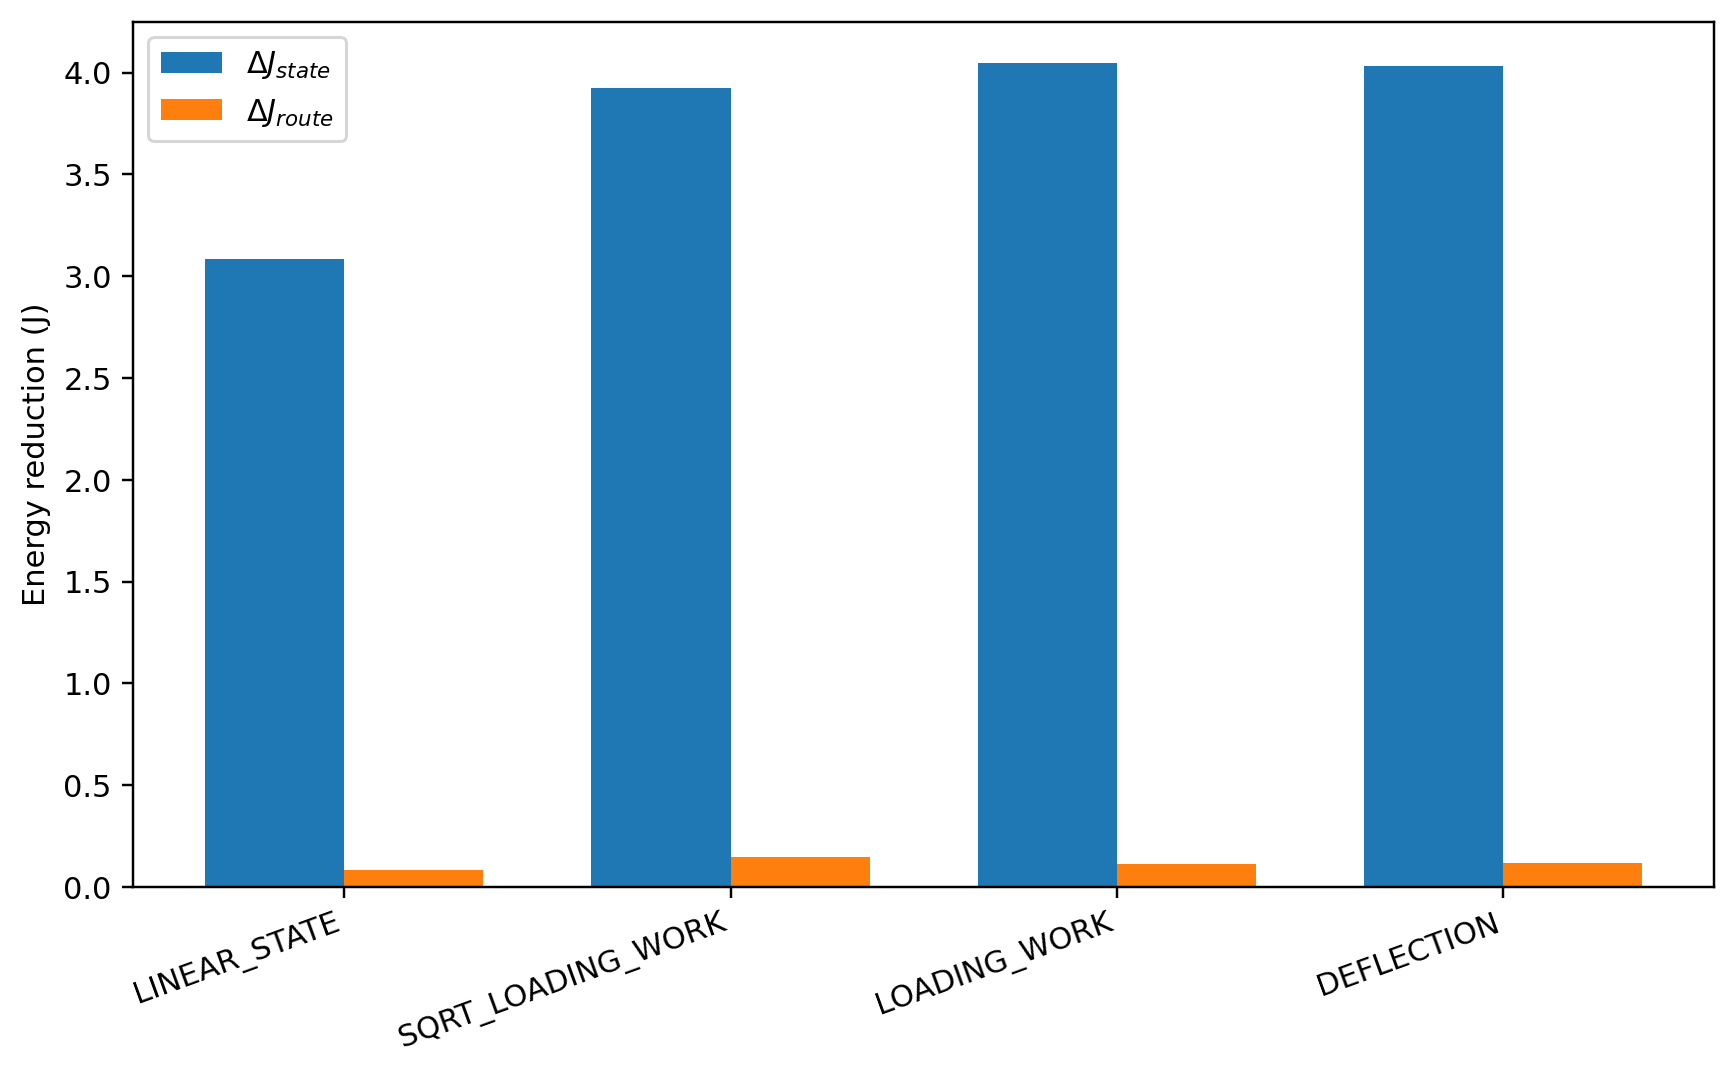
\includegraphics[width=0.78\linewidth]{figure_state_vs_route.png}
\caption{Decomposition of adaptive benefit into state-adaptation and rerouting contributions for the corrected representative 2-D heterogeneous map.}
\label{fig:state_route}
\end{figure}

\subsection{Spatial-ensemble results}
A controlled 2-D ensemble tested two terrain pairs, three terrain-B fractions, random and clustered arrangements, ten map realizations per condition, four baseline rolling-resistance values, three state-dependent rolling-loss amplitudes, and four rolling-loss model forms.

Terrain composition alone did not determine adaptive benefit. For HARD\_GROUND/JLU\_MARS1\_LOOSE at 50\% terrain B, the median benefit increased from 0.090 for random layouts to 0.331 for clustered layouts. At 75\% terrain B, however, the ordering reversed slightly: 0.186 for random layouts and 0.142 for clustered layouts. Spatial clustering therefore did not have a monotonic effect.

The terrain-pair contrast also mattered. At 50\% terrain B under clustered arrangement, HARD\_GROUND/JLU\_MARS1\_LOOSE had median \(B_{\mathrm{ideal}}=0.331\), whereas JLU\_MARS1\_DENSE/JLU\_MARS1\_LOOSE had median \(B_{\mathrm{ideal}}=0.053\). This is consistent with the proposed mechanism that greater incompatibility between locally preferred compliance states provides more opportunity for adaptation to outperform a global fixed compromise.

\begin{figure}[htbp]
\centering
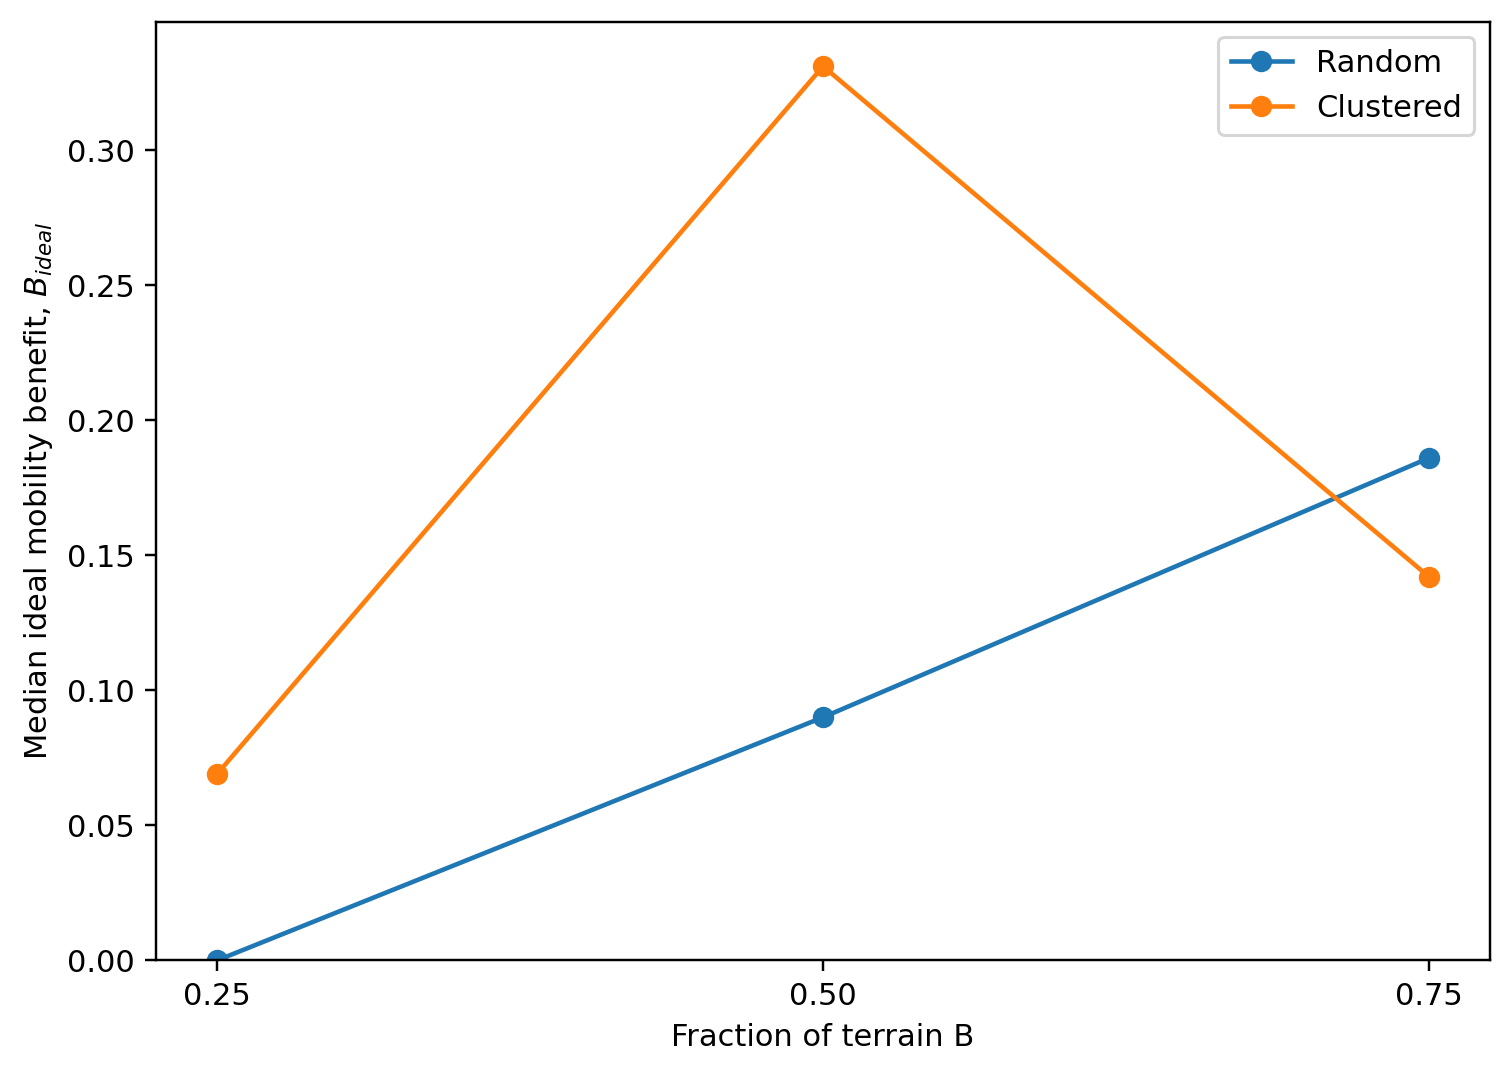
\includegraphics[width=0.76\linewidth]{figure_ensemble_median_hard_loose.png}
\caption{Median ideal mobility benefit versus terrain-B fraction for HARD\_GROUND/JLU\_MARS1\_LOOSE maps.}
\label{fig:ensemble_hard_loose}
\end{figure}

\begin{figure}[htbp]
\centering
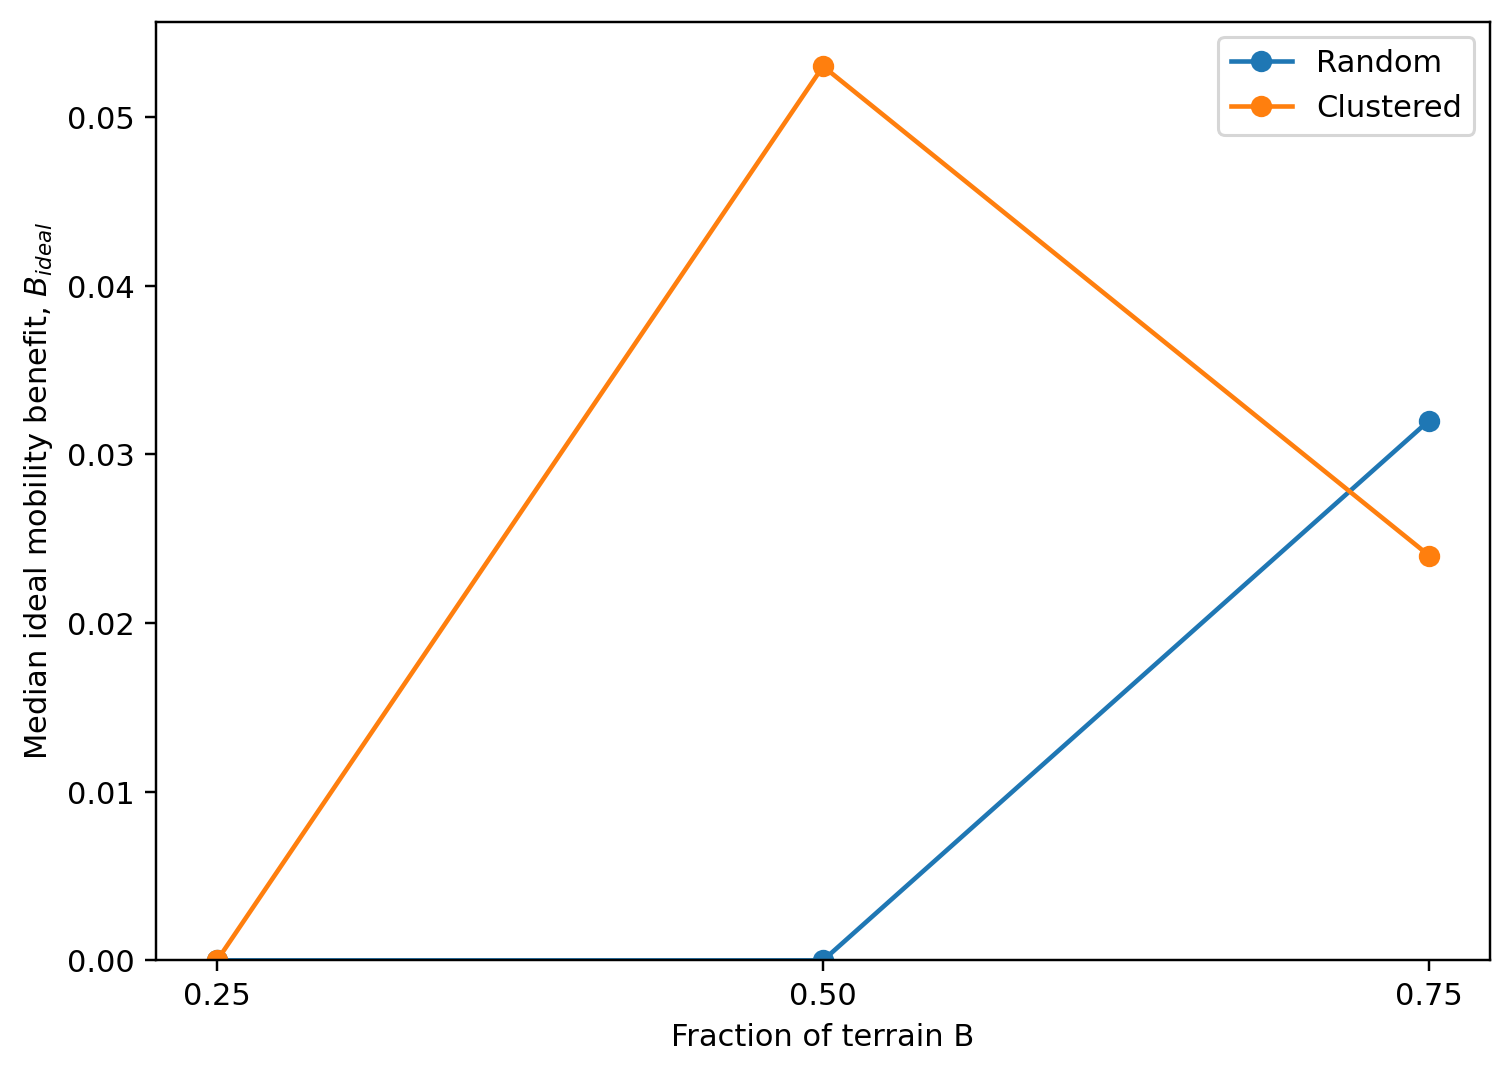
\includegraphics[width=0.76\linewidth]{figure_ensemble_median_dense_loose.png}
\caption{Median ideal mobility benefit versus terrain-B fraction for JLU\_MARS1\_DENSE/JLU\_MARS1\_LOOSE maps.}
\label{fig:ensemble_dense_loose}
\end{figure}

\subsection{Benefit is conditional rather than automatic}
Several conditions contained zero-benefit cases. For random hard/loose maps at 25\% terrain B, median benefit was zero and only 10\% of the deterministic cases were positive. For random dense/loose maps at the same terrain fraction, only 8.3\% were positive. At 75\% terrain B, both hard/loose arrangements were positive in all tested deterministic cases, while the dense/loose pair was positive in 83.3\% of cases. These are frequencies over the selected synthetic ensemble and sensitivity set, not real-world probabilities.

\begin{figure}[htbp]
\centering
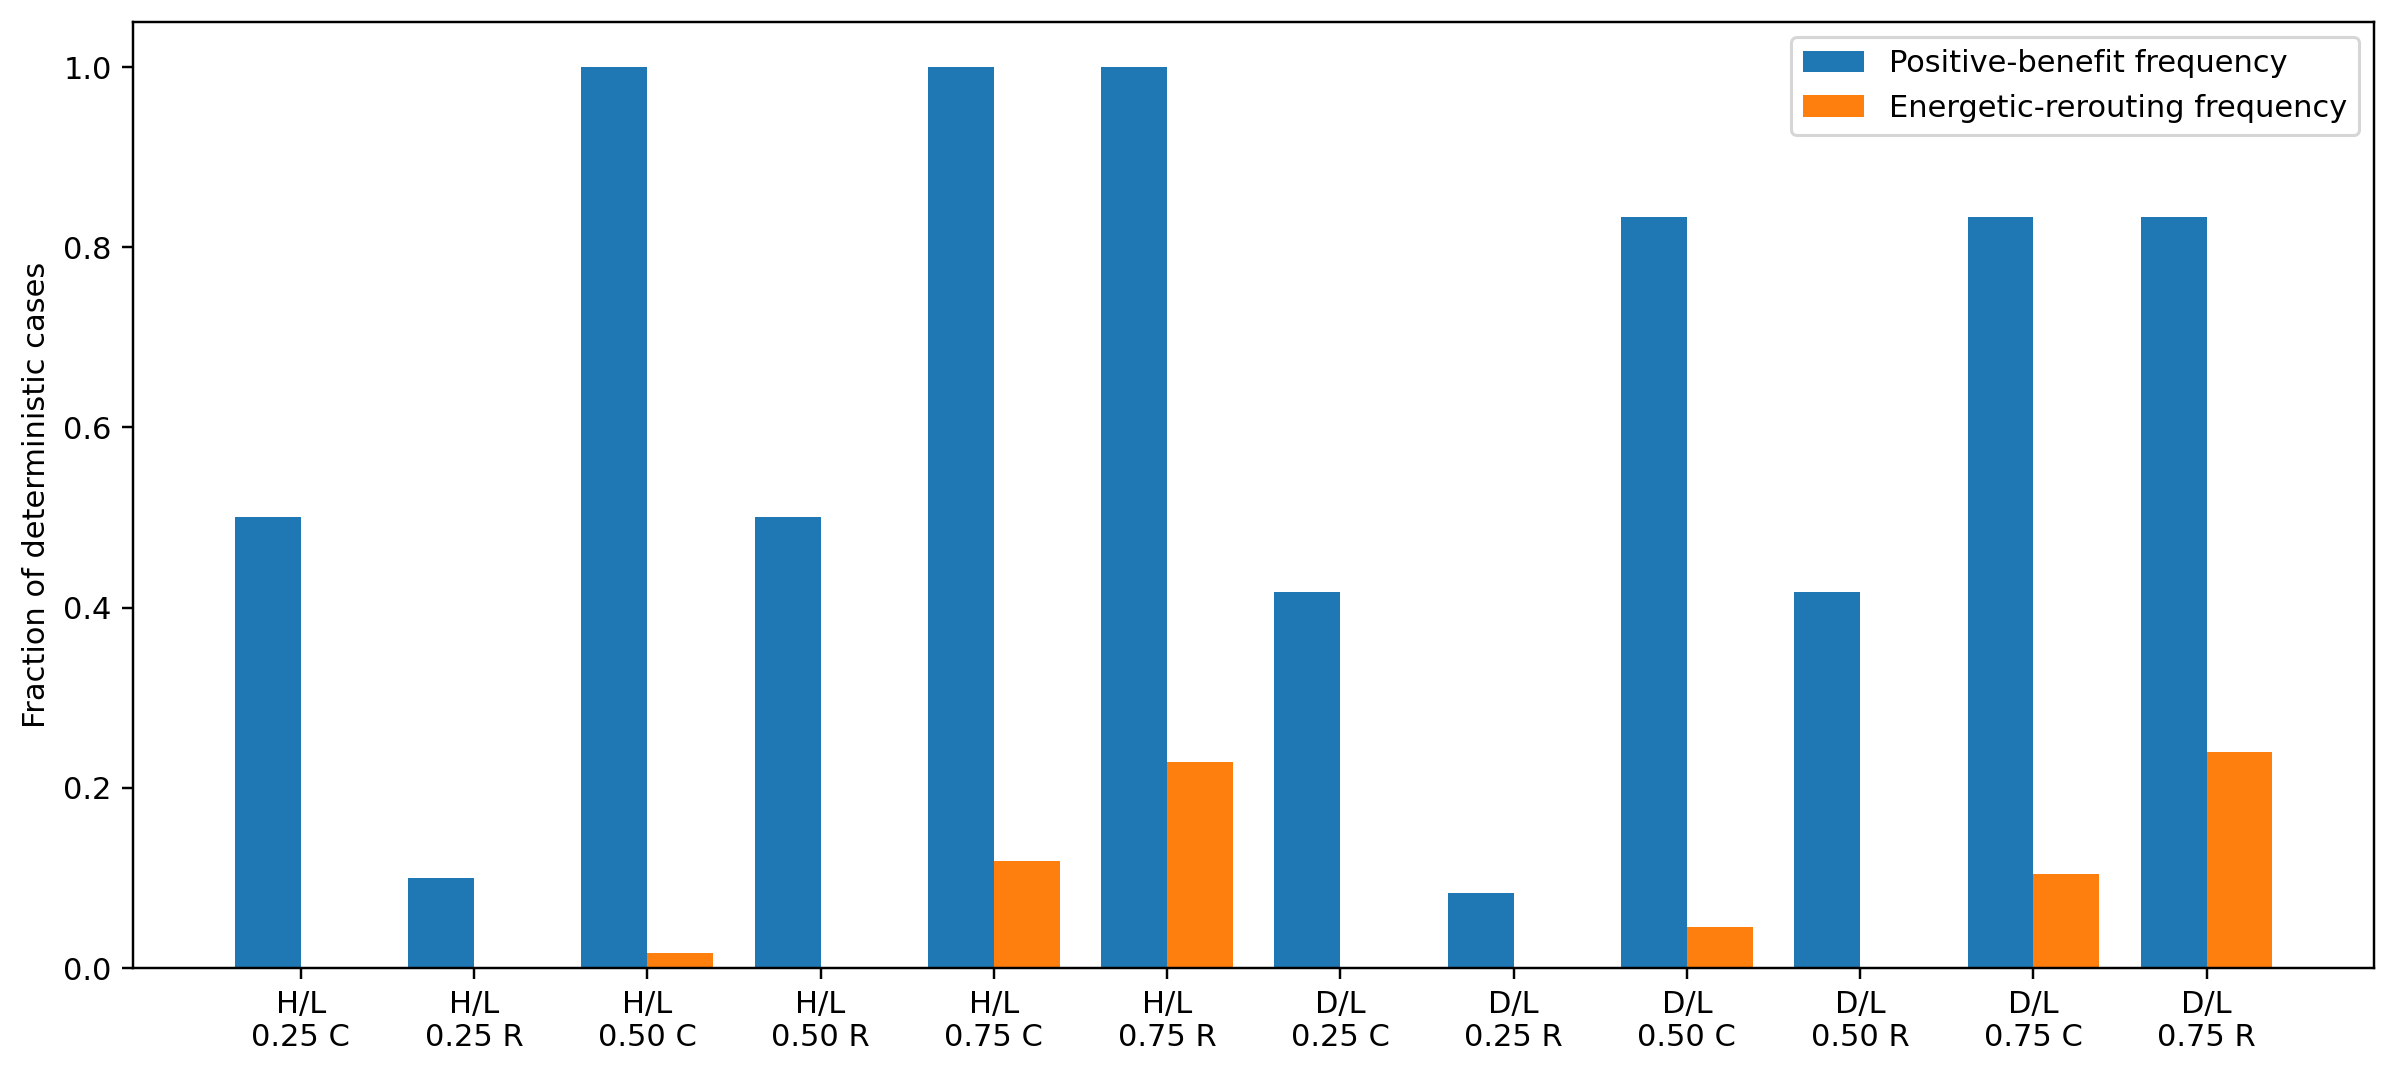
\includegraphics[width=0.96\linewidth]{figure_ensemble_case_frequencies.png}
\caption{Fraction of deterministic ensemble cases with positive ideal benefit and with nonzero energetic rerouting contribution.}
\label{fig:ensemble_frequencies}
\end{figure}

\subsection{Range of outcomes}
The full ensemble produced broad ranges of \(B_{\mathrm{ideal}}\) within several conditions, reflecting both map realization and rolling-loss sensitivity. The largest hard/loose range was approximately 0 to 0.767, whereas the dense/loose ensemble remained below approximately 0.164 in the reported summary. These ranges are deterministic sensitivity envelopes, not confidence intervals.

\begin{figure}[htbp]
\centering
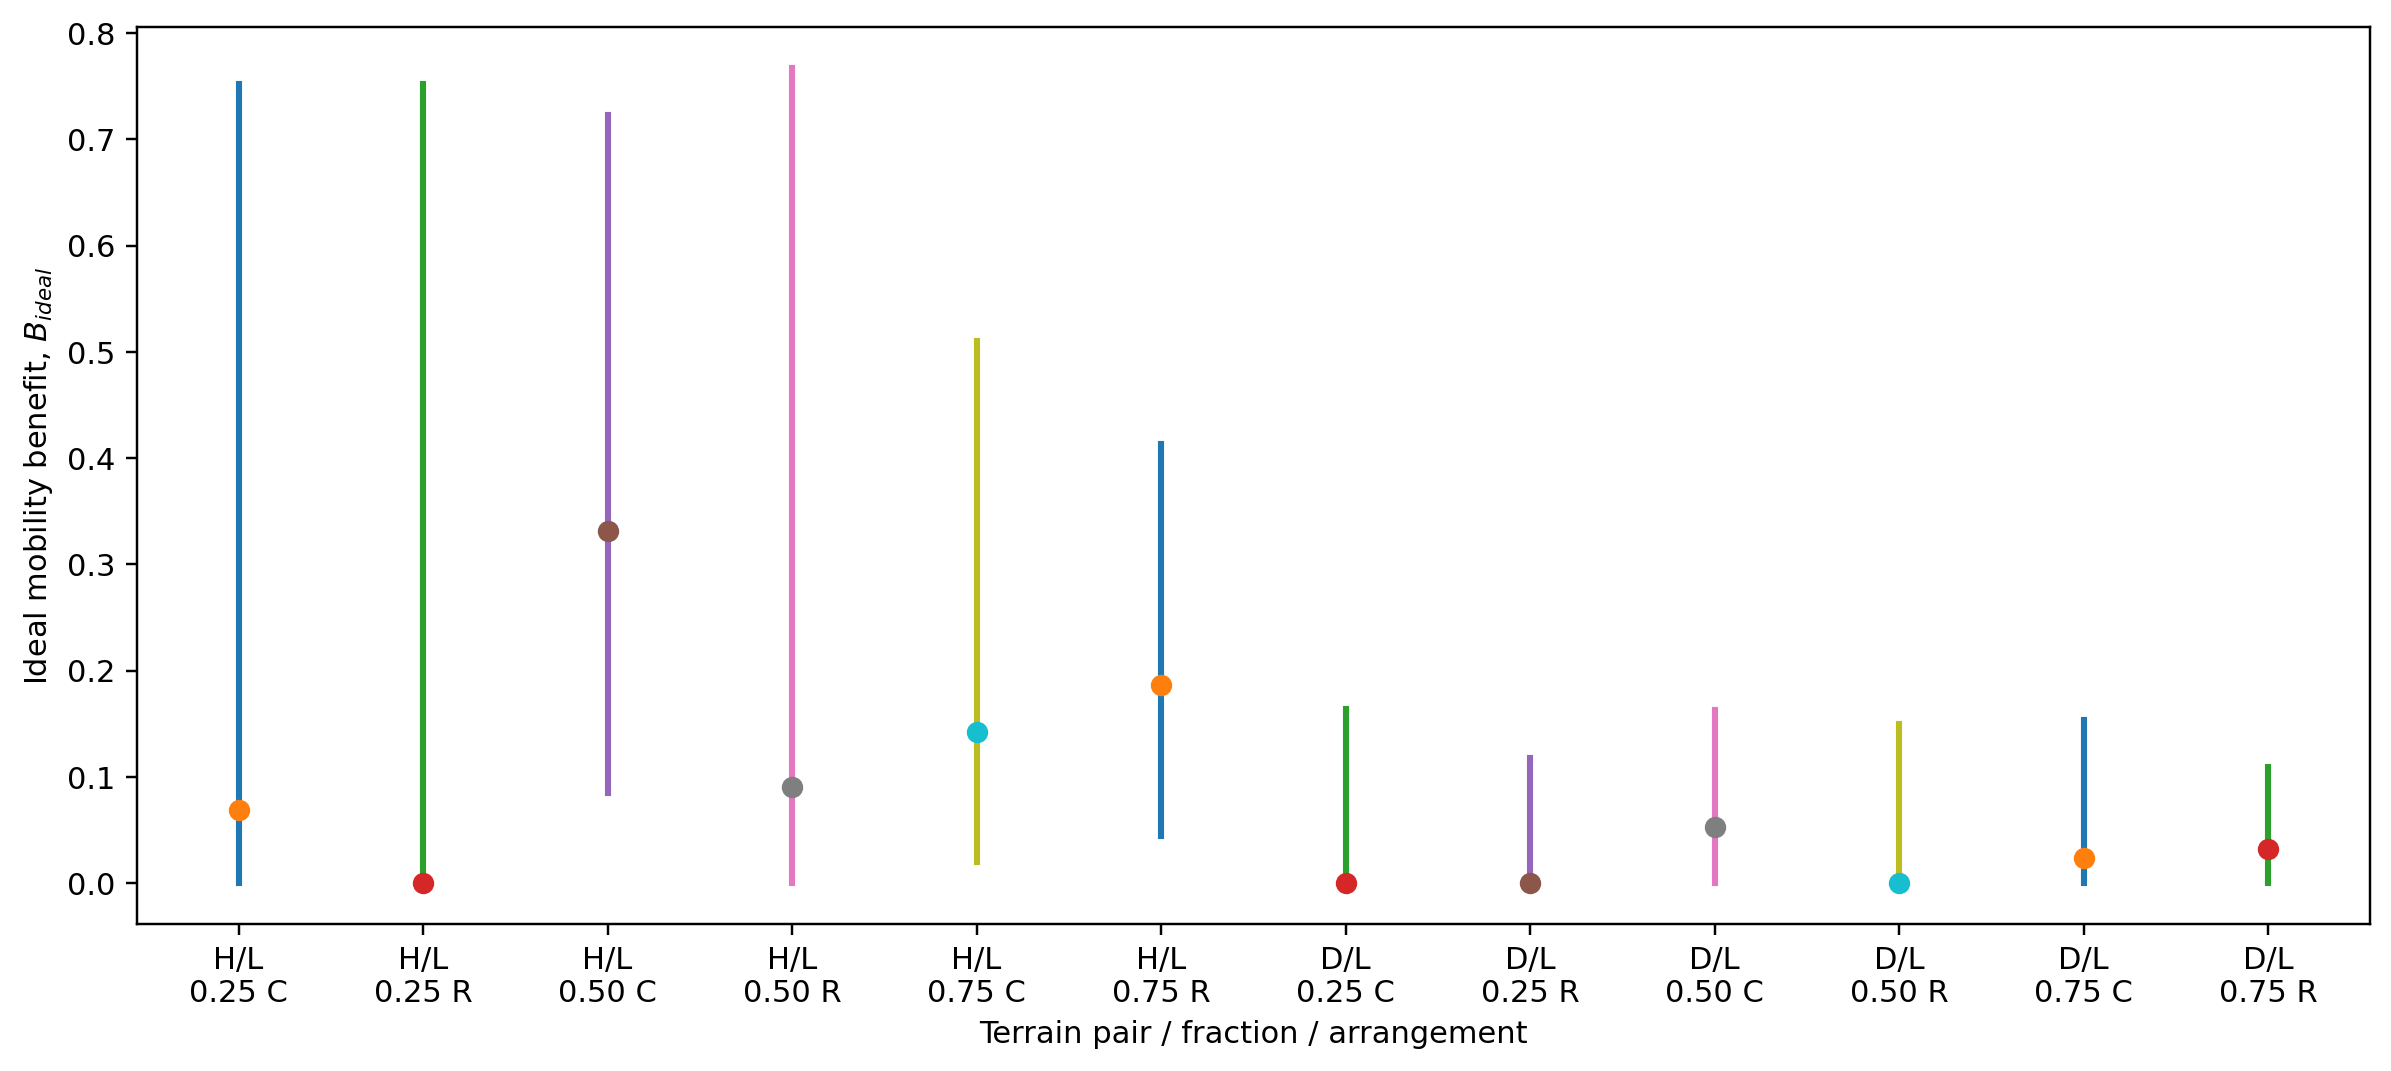
\includegraphics[width=0.98\linewidth]{figure_ensemble_ranges.png}
\caption{Minimum, median, and maximum ideal mobility benefit for each terrain-pair, terrain-fraction, and arrangement condition.}
\label{fig:ensemble_ranges}
\end{figure}

\subsection{Rerouting frequency}
Energetic rerouting was counted only when \(\Delta J_{\mathrm{route}}>0\), rather than from a route-coordinate change alone. The largest reported rerouting frequency was 24.0\% for random dense/loose maps at 75\% terrain B, followed by 22.9\% for random hard/loose maps at the same fraction. The median route-share statistic was nevertheless zero in every ensemble group because more than half of the cases in each group had no energetic rerouting contribution. Rerouting is therefore map-architecture dependent rather than universally dominant or negligible.

\subsection{Obstacle-feasibility validation}
The obstacle model was tested at every exact Lee-tested height represented in the source data. The first admissible numerical compliance states were 0.43, 0.58, 0.58, 0.58, 0.75, 1.00, 1.00, and 1.00 for obstacle heights 90, 95, 100, 105, 110, 115, 120, and 125 mm, respectively. The regression passed for all four rolling-loss model forms. These values validate the implementation of the source-derived feasibility mapping; no obstacle-energy term is inferred.

\begin{figure}[htbp]
\centering
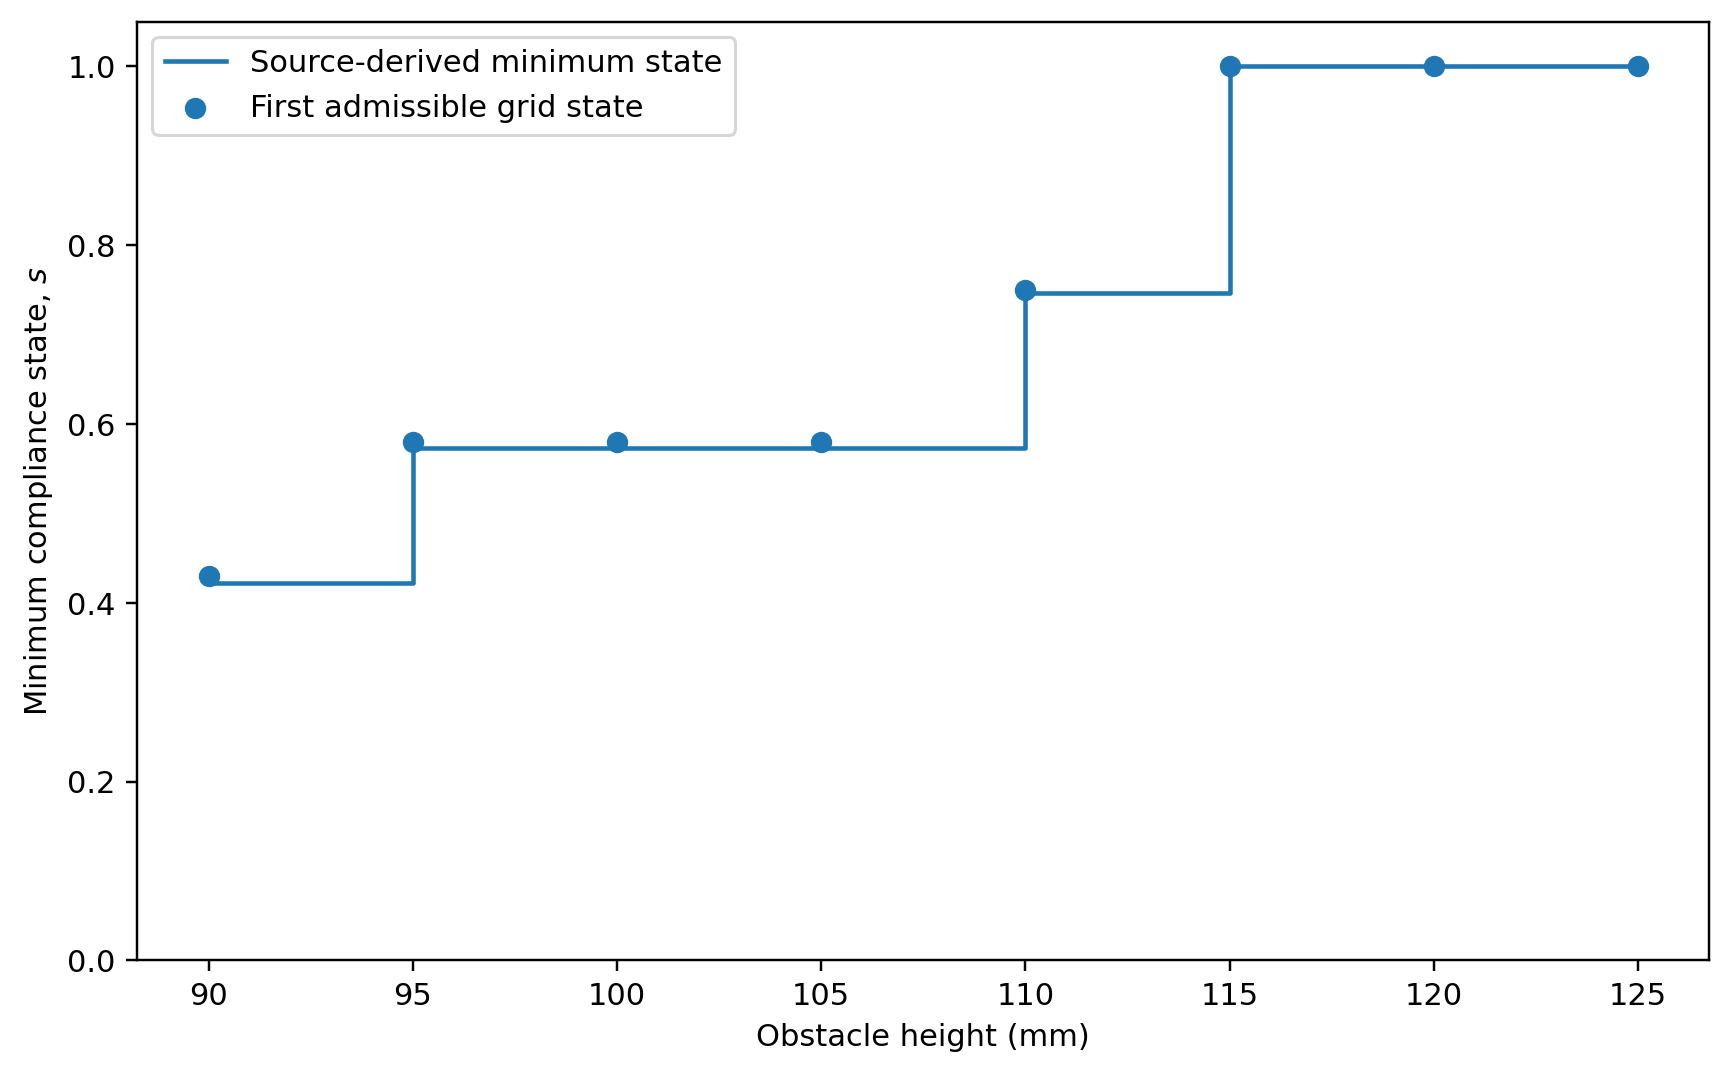
\includegraphics[width=0.76\linewidth]{figure_obstacle_thresholds.png}
\caption{Source-derived minimum compliance threshold and first admissible numerical state for each exact Lee-tested obstacle height.}
\label{fig:obstacle_thresholds}
\end{figure}

\subsection{Interpretation}
Taken together, the results support three conclusions. First, adaptive compliance does not guarantee benefit; homogeneous and weak-contrast conditions can yield zero benefit. Second, positive benefit emerges most consistently when relevant terrain classes have sufficiently different compliance preferences. Third, the magnitude of the predicted benefit depends materially on both spatial terrain organization and the uncalibrated compliance-dependent rolling-loss model. The present results therefore support a conditional ideal mobility advantage while the exact magnitude of \(B_{\mathrm{ideal}}\) should remain a sensitivity result rather than a calibrated mission prediction.

\section{Limitations}

The final interpretation is subject to the following limitations:
\begin{enumerate}[label=(\arabic*)]
\item the present wheel constitutive calibration is tied to the Lee small-wheel geometry and supported load domain;
\item a full multi-wheel rover load-distribution model is not included;
\item suspension, steering, turning radius, full rover footprint, and body clearance are not modeled;
\item 8-neighbor routing retains finite angular anisotropy;
\item no calibrated cyclic rolling-loss law is available;
\item no calibrated slip-energy model is included;
\item state-transition energy is set to zero to isolate ideal mobility benefit;
\item downhill regeneration and braking losses are not modeled;
\item obstacle data are used only for feasibility;
\item synthetic terrain maps are methodological test cases rather than statistical mission-terrain samples;
\item some inherited soil parameter sets require final provenance audit before formal publication;
\item generalization to a broader wheel family requires validated scaling of $D(F,s)$ with geometry and load.
\end{enumerate}

\section{Research development summary}

The project began as a simple route-optimization comparison between soft and stiff wheel states on heterogeneous terrain. It was progressively rebuilt around experimentally recoverable information from Lee et al.: the wheel was represented by a continuous compliance coordinate and force--deformation surface, the small-wheel geometry and nominal load were corrected, and obstacle measurements were restricted to feasibility rather than converted into invented energy penalties. Reduced Bekker--Wong terramechanics was coupled to compliance-dependent contact geometry, slope, and traction feasibility. Intermediate formulations were rejected when audits exposed state-mapping errors, arbitrary penalties, nearest-state artifacts, destination-only edge-cost bias, grid-resolution effects, and Manhattan routing bias. The final optimizer compares the globally optimal fixed state and route with a fully adaptive state sequence and route, while decomposing savings into state-adaptation and rerouting contributions. Negative controls, obstacle-threshold regressions, slope checks, deterministic rolling-loss sensitivity studies, grid-convergence tests, and connectivity audits were used throughout. The resulting framework is numerically well characterized, while its largest unresolved physical uncertainty---compliance-dependent rolling loss---is deliberately retained as a sensitivity envelope rather than treated as calibrated.

\section{Final interpretation}

The present work establishes a source-informed and numerically audited framework for determining when variable compliance can provide an ideal mobility advantage over the best fixed-compliance wheel. The model is most useful at this stage for identifying mechanisms, tradeoffs, and sensitivity to terrain heterogeneity. It should not yet be interpreted as a mission-calibrated energy predictor or as a validated constitutive model for an arbitrary variable-compliance wheel family.

\begin{thebibliography}{9}
\bibitem{Lee2024}
J.-Y. Lee et al., ``Variable-stiffness--morphing wheel inspired by the surface tension of a liquid droplet,'' \emph{Science Robotics}, vol. 9, no. 93, eadl2067, 2024. doi: 10.1126/scirobotics.adl2067.

\bibitem{Bekker1969}
M. G. Bekker, \emph{Introduction to Terrain-Vehicle Systems}. University of Michigan Press, 1969.

\bibitem{Wong2001}
J. Y. Wong, \emph{Theory of Ground Vehicles}, 3rd ed. John Wiley \& Sons, 2001.

\bibitem{Wong2010}
J. Y. Wong, \emph{Terramechanics and Off-Road Vehicle Engineering: Terrain Behaviour, Off-Road Vehicle Performance and Design}, 2nd ed. Elsevier, 2010.

\bibitem{Shen2024}
Y. Shen, M. Zou, H. Cao, D. Pan, B. Yuan, and L. He, ``Current-Based Analysis and Validation of a Wheel--Soil Interaction Model for the Trafficability of a Planetary Rover,'' \emph{Aerospace}, vol. 11, no. 11, p. 892, 2024. doi: 10.3390/aerospace11110892.
\end{thebibliography}
\end{document}
